%%%%%%%%%%%%%%%%%%%%%%%%%%%%%%%%%%%%%%%%%%%%%%%%%%%%%%%%%%%%%%%%%%%%%%
%%                                                                 %%
%% Please do not use \input{...} to include other tex files.       %%
%% Submit your LaTeX manuscript as one .tex document.              %%
%%                                                                 %%
%% All additional figures and files should be attached             %%
%% separately and not embedded in the \TeX\ document itself.       %%
%%                                                                 %%
%%%%%%%%%%%%%%%%%%%%%%%%%%%%%%%%%%%%%%%%%%%%%%%%%%%%%%%%%%%%%%%%%%%%%

% References live in uaere.bib and are called with \bibliography.
% Draft. Do not post to arXiv until a patent provisional is filed.

%%\documentclass[referee,sn-basic]{sn-jnl}% referee option is meant for double line spacing

%%=======================================================%%
%% to print line numbers in the margin use lineno option %%
%%=======================================================%%

%%\documentclass[lineno,sn-basic]{sn-jnl}% Basic Springer Nature Reference Style/Chemistry Reference Style

%%======================================================%%
%% to compile with pdflatex/xelatex use pdflatex option %%
%%======================================================%%

%%\documentclass[pdflatex,sn-basic]{sn-jnl}% Basic Springer Nature Reference Style/Chemistry Reference Style

%%\documentclass[sn-basic]{sn-jnl}% Basic Springer Nature Reference Style/Chemistry Reference Style
\documentclass[sn-mathphys-num]{sn-jnl}% Math and Physical Sciences Numeric Reference Style

% Fast compile toggle: set true while editing, false for camera-ready build
\newif\iffastcompile
\fastcompilefalse
\iffastcompile
  \PassOptionsToPackage{draft}{graphicx}
\fi
%%\documentclass[sn-aps]{sn-jnl}% American Physical Society (APS) Reference Style
%%\documentclass[sn-vancouver]{sn-jnl}% Vancouver Reference Style
%%\documentclass[sn-apa]{sn-jnl}% APA Reference Style
%%\documentclass[sn-chicago]{sn-jnl}% Chicago-based Humanities Reference Style
%%\documentclass[sn-standardnature]{sn-jnl}% Standard Nature Portfolio Reference Style
%%\documentclass[default]{sn-jnl}% Default
%%\documentclass[default,iicol]{sn-jnl}% Default with double column layout

%%%% Standard Packages
\usepackage[T1]{fontenc}
\usepackage{tabularx}
\usepackage{enumitem}
\usepackage{graphicx}
\usepackage{array,colortbl,xcolor,longtable}
\usepackage{mathtools}
% \usepackage{amsmath}
\usepackage{amssymb}
\usepackage{makecell}
\usepackage{lscape}
\usepackage{lipsum}
\usepackage{float}
\usepackage{optidef}
\usepackage[section]{placeins}
\usepackage{algorithm}
\usepackage{braket}
\usepackage{algpseudocode}
\usepackage{newtxtext,newtxmath}
\usepackage[scaled=1.0]{rsfso}
%\DeclareMathAlphabet{\mathscr}{U}{rsfso}{m}{n}
\usepackage{color,soul}
\usepackage{pifont}% http://ctan.org/pkg/pifont
\newcommand{\cmark}{\ding{51}}%
\newcommand{\xmark}{\ding{55}}%

% Float tuning: keep figures/tables near references without forcing large white gaps
\setcounter{topnumber}{3}
\setcounter{bottomnumber}{2}
\setcounter{totalnumber}{5}
\renewcommand{\topfraction}{0.9}
\renewcommand{\bottomfraction}{0.8}
\renewcommand{\textfraction}{0.07}
\renewcommand{\floatpagefraction}{0.8}

\theoremstyle{thmstyleone}%
\newtheorem{theorem}{Theorem}%
\newtheorem{proposition}[theorem]{Proposition}%

\theoremstyle{thmstyletwo}%
\newtheorem{example}{Example}%
\newtheorem{remark}{Remark}%

\theoremstyle{thmstylethree}%
\newtheorem{definition}{Definition}%

\raggedbottom
\hbadness=10000
\vbadness=10000
\hfuzz=6pt

\begin{document}

\title[Explanation gating under an energy-cost model]{Uncertainty-Aware Event-Level Trust Gating for Energy-Efficient Underwater Acoustic Event Classification}

\author[1]{\fnm{Rhutvik} \sur{Hegde}}

\author[1]{\fnm{Kalyani} \sur{Manoj}}

\author*[1]{\fnm{Shashank Mouli} \sur{Satapathy}}

\affil[1]{\orgdiv{School of Computer Science and Engineering}, \orgname{Vellore Institute of Technology}, \orgaddress{\city{Vellore}, \postcode{632014}, \state{Tamil Nadu}, \country{India}}}

\abstract{This study examines whether uncertainty and contextual terms improve event-level explanation gating over a confidence threshold under an explicit energy-cost model. The label is a class-balanced logistic on a pre-segmented window and is emitted whether or not the explanation runs. A hand-set sigmoid, called event trust, combines wake confidence with sensor health, an environmental term, and a Dirichlet uncertainty. Trust is a gate score, not a calibrated probability that the label is correct. A validation percentile of that score chooses between stopping at Level~1 and paying for a Level-3 explanation. On three recording-locked seeds of the public Pamlico oyster-toadfish candidates, macro-F1 is $0.844 \pm 0.004$ and does not depend on the gate. Health, environment, and epistemic uncertainty are constant on these files, so the trust score ranks windows in the same order as wake confidence and selects the same test windows. The uncertainty-only gate does not: it also explains confident negatives. Relative to always running Level~3, a datasheet model estimates a saving of $10.4\% \pm 0.7\%$ only when the selected path is charged for a Level-2 computation that does not produce the label. The clips are pre-segmented candidates from one estuary. A 16-species Watkins tape hold-out reaches macro-F1 $0.281$ and misses a pre-registered bar of $0.70$. That result is not generalisation. The energy figures are model estimates, not measured power and not an underwater deployment.}

\keywords{Underwater acoustics, explanation gating, selective inference, confidence threshold, energy-cost model, oyster toadfish}

\maketitle

\section{Introduction}\label{sec:intro}

\subsection{Background and motivation}\label{sec:background}

Passive acoustic monitoring spends its energy in the instrument that digitizes the sea, and only afterwards in any classifier. A fixed installation is either a cabled hydrophone or an autonomous recorder that writes to its own memory and is recovered later \cite{mellinger2007,sousalima2013}. The sensor is passive: it does not project sound at the animal \cite{zimmer2011}. Continuous broadband recording keeps short calls and fills disks. A programmed duty cycle stretches a battery and drops every call that falls in an off interval \cite{wiggins2007,wiggins2023}. A classifier that runs on shore, months later, never sees the joules that choice already spent.

The recorders that produced the literature's long archives set the scale. A single-channel HARP at 200\,kHz draws about 0.5\,W while it writes \cite{wiggins2023}. Earlier HARP descriptions put the hydrophone near 50\,mW and the logger near 250\,mW, with a large extra cost while disks spin \cite{wiggins2007}. Compact recorders and click loggers occupy a different point on the same trade: less bandwidth, a smaller housing, and a detector that is part of the instrument rather than a later computer \cite{taylor2024,todd2023,ivanchikova2023}. Turning a recording into a habitat metric is a separate measurement problem \cite{merchant2015}. Ambient spectra are the background of that recording \cite{knudsen1948,wenz1962,hildebrand2009}. None of those watts is the millijoule cost of an explanation on a sample that has already been stored. A software gate does not replace the recorder.

The call used for the main experiment is the oyster toadfish boatwhistle. The fundamental sits near 80--220\,Hz and the call lasts a few hundred milliseconds \cite{gray1961,fine1978,elemans2014,mensinger2014}. The public candidate set that accompanies the ToadFishFinder catalog was recorded in Pamlico Sound, template-matched, and released as 1.35\,s clips at 24\,kHz \cite{bohnenstiehl2023,bohnenstiehl2023data}. This paper scores the centre 1.0\,s of those clips at 16\,kHz. It does not discover events in a continuous stream.

\subsection{Problem statement}\label{sec:problem}

The decision studied here is narrower than classifying the ocean. For each already cut window, a cheap head has already produced a label. The question is whether uncertainty and contextual terms improve the further choice to attach a costly explanation, relative to a threshold on wake confidence, under a stated energy-cost model. The implemented action is binary. If the score is at least $\tau$, run Level~3. Otherwise stop at Level~1. The label is emitted in both cases. Gating does not change classification accuracy.

Acceptance of a label, escalation to a heavier model, and abstention are different actions. This system implements the choice to run or skip the explanation. A separate abstention baseline, which refuses the label, is reported under its own name. It is not the source of the macro-F1 above.

\subsection{Research gap}\label{sec:gap}

A confidence threshold is the natural baseline for this decision, and it has two properties that are easy to blur. It is not, by itself, a calibrated probability that the label is correct. A threshold chosen on the test set, or a search that sees the test labels, reports an operating point the node did not have when the window arrived. Extra terms can matter when the node is unhealthy, when the sea state changes, or when a peaked probability falls on the negative class. On the corpus in this paper those extra terms do not vary, so they cannot be claimed as a demonstrated improvement. The experiment asks whether they help anyway.

Published trust models for underwater acoustic networks answer a different question. They score whether a node is faulty, selfish, or compromised, and they reweight that node in routing or fusion \cite{signori2022,song2025,he2024,xia2026,akyildiz2005}. Ship and animal classifiers answer which class produced a clip that was already cut out \cite{irfan2021,bohnenstiehl2023,hagiwara2022}. Those lines are context. They are not the comparison.

\subsection{Research objectives and contributions}\label{sec:contributions}

The objective is to run that comparison on the available recordings and to state what it shows, including where the proposed score adds nothing.

The contributions that the experiments support are three.
\begin{enumerate}[leftmargin=1.5em]
\item On the two-class toadfish corpus, event trust does not outperform a confidence threshold. After each score's own validation threshold, the two gates select the same windows. An uncertainty-only gate explains confident negatives and is less selective. The equivalence is the finding. It is not a claim that the extra terms improve the decision.
\item A cost account of that decision. The reported saving against always running Level~3 exists only when the selected path is charged for a Level-2 budget the logistic does not execute. Sensitivity to that assumption is part of the result. The joules are a datasheet model, not a deployment measurement.
\item A matched protocol: one validation rule for every score, abstention reported separately from explanation gating, and intervals whose unit is the seed.
\end{enumerate}
The hand-set score is the object of the comparison. It is not, on these files, a better gate. The knowledge graph explains a predicted class. It is not a contribution to detection or to the trust score.

\section{Related work}\label{sec:related}

\subsection{Underwater acoustic event classification}\label{sec:rw-class}

Ship-radiated-noise benchmarks such as DeepShip score vessel class on clips that have already been cut from a recording \cite{irfan2021}. Bioacoustic catalogs score calls the same way. Bohnenstiehl's ResNet-50 and SVM remain the specialist result on the Pamlico toadfish candidates \cite{bohnenstiehl2023}. This paper uses a class-balanced logistic on log-Mel statistics plus three band numbers, and it does not claim to beat that specialist. The Watkins Marine Mammal Sound Database is a library of isolated, identified cuts gathered over decades and instruments \cite{sayigh2016}. Random splits of the small best-of subset, as in BEANS \cite{hagiwara2022}, and date-and-location or tape hold-outs \cite{aguiar2021} are different tasks. Section~\ref{sec:robust} reports a tape hold-out and does not compare its macro-F1 with the toadfish macro-F1.

\subsection{Energy-aware and selective inference}\label{sec:rw-energy}

Duty-cycled recorders save energy by not acquiring \cite{wiggins2007,wiggins2023,vanparijs2009,baumgartner2019}. A compute gate on a window that has already been digitized saves a different, and much smaller, quantity.

The closest decision rules are confidence-based. Selective classification refuses the label when confidence is below a threshold \cite{geifman2017}. Early-exit networks skip later layers when an intermediate classifier is already confident \cite{teerapittayanon2016}. Both spend less computation on easy inputs. Neither is the rule in this paper. Selective classification changes which labels are emitted. Early exit changes how deep the classifier runs. Here the label is always the logistic, and the threshold decides only whether an explanation is attached. The confidence row in Section~\ref{sec:compare} is that narrower rule. The abstention baseline, reported separately, is the selective-classification action. An always-cheap path never explains. An always-expensive path always does. Both use the same logistic label.

\subsection{Uncertainty-aware classification and trust estimation}\label{sec:rw-uncertainty}

Network trust estimates a node or a link and is used for routing or fusion, not for a per-window explanation \cite{signori2022,song2025,he2024,xia2026}. Sensoy, Kaplan, and Kandemir map evidence to a Dirichlet and read epistemic uncertainty from the total concentration \cite{sensoy2018}. This paper does not train that loss. It lifts a fitted logistic with a fixed concentration of 20, which makes the epistemic term constant on a two-class head. A hand-written graph can state a cause after the label is chosen \cite{traer2021,olvera2025,dung1995}. It is not an input to the gate score.

\subsection{What the comparison is}\label{sec:novelty}

Table~\ref{tab:gap} places the implemented baselines next to the nearest published lines. Cells describe what those papers and this code actually do. The graph is not listed as context inside the trust score, because Section~\ref{sec:trust} does not use it as an input.

\begin{table}[!htbp]
\centering
\caption{What is and is not in the decision. Cells describe the cited papers and the gates implemented in this study.}
\label{tab:gap}
\footnotesize
\setlength{\tabcolsep}{3pt}
\begin{tabular}{|p{3.4cm}|p{2.5cm}|p{2.7cm}|p{2.5cm}|p{2.0cm}|}
\hline
\textbf{Approach} & \textbf{Uncertainty in the score} & \textbf{Health or environment in the score} & \textbf{What the threshold does} & \textbf{Unit} \\
\hline
Node or channel trust \cite{signori2022,song2025,he2024,xia2026} & No event-uncertainty model & Channel or neighbour, not this score & Routing or fusion & Node \\
\hline
Selective classification \cite{geifman2017} & No & No & Refuses the label & Sample \\
\hline
Early exit \cite{teerapittayanon2016} & No & No & Skips later layers of the classifier & Sample \\
\hline
Clip classifier \cite{irfan2021,bohnenstiehl2023} & No & No & No threshold & Clip \\
\hline
Dirichlet head \cite{sensoy2018} & Yes, from a trained concentration & No & No threshold & Class distribution \\
\hline
Confidence threshold (implemented) & No separate term & No & Level 3 or Level 1; label kept & Window \\
\hline
Uncertainty threshold (implemented) & Yes, inverted & No & Level 3 or Level 1; label kept & Window \\
\hline
Confidence--uncertainty (implemented) & Yes & Weights set to 0 & Level 3 or Level 1; label kept & Window \\
\hline
Event trust (implemented) & Yes; epistemic part constant here & Yes, and both constant here. The graph is not an input & Level 3 or Level 1; label kept & Window \\
\hline
\end{tabular}
\end{table}

The comparison is one validation-chosen threshold and one cost model, applied to each scalar. Section~\ref{sec:results} shows that, on these files, event trust selects the same windows as the confidence threshold, and that the uncertainty threshold does not.

\section{Problem formulation and system framework}\label{sec:framework}

\subsection{System model and assumptions}\label{sec:model}

A window is 1.0\,s at 16\,kHz, taken from the centre of a longer clip. Integer PCM is divided by full scale, $2^{31}$ for 32-bit and 32768 for 16-bit. IEEE-float samples are kept as stored. Training clips are not peak-normalised. The environment state carries temperature, salinity, depth, sea state, turbulence, and a sound speed \cite{mackenzie1981}. The sensor state carries clipping, drift, ADC width, and a fault class. The Pamlico release has no conductivity-temperature-depth cast and no health log. Every fish window uses one imputed state: 12\,$^{\circ}$C, 34\,PSU, 40\,m, sea state 2, turbulence 0.1, and a healthy sensor. Sea state 2 is a constant.

Level~0 is an FFT surprise against a Knudsen/Wenz ambient \cite{knudsen1948,wenz1962}. A logistic map with center 8 and scale 1.5 crosses an admit value of 0.15 at surprise 5.398. There is no test of the form ``if energy exceeds a threshold.'' A head that stores biological labels records surprise and does not sleep on that cutoff. A ship head, which has no label list, still returns a reject when admit is low. The fish experiments in Section~\ref{sec:results} always run the logistic, so Level~0 does not change their labels.

A separate simulation, described in Appendix~\ref{app:twin}, uses a different generator. It is not a Pamlico recording and it is not the energy result of the fish experiment.

\subsection{Problem formulation}\label{sec:formulation}

For window $i$, the logistic produces a class distribution. From it the node computes wake confidence $C_i$, aleatoric uncertainty $U_i^{(a)}$, and epistemic uncertainty $U_i^{(e)}$. Health consistency $\kappa_i$ and environmental consistency $\rho_i$ are the other two scalars defined in Section~\ref{sec:trust}. The trust score $T_i$ is a function of those scalars. The implemented decision is
\begin{equation}
a_i = g(T_i) =
\begin{cases}
\text{Level 3 explanation} & \text{if } T_i \ge \tau, \\
\text{Level 1 label only} & \text{if } T_i < \tau.
\end{cases}
\label{eq:decision}
\end{equation}
The label $\hat{y}_i$ does not depend on $a_i$. The cost of window $i$ does. Section~\ref{sec:energy} writes that cost as $E_i = E_{a,i} + E_{g,i} + E_{p,i}$. The threshold $\tau$ is chosen on validation only, by the rule in Section~\ref{sec:policy}. The same rule is applied to every competing score, so the trust gate does not receive extra degrees of freedom.

\subsection{Overview of the proposed framework}\label{sec:overview}

Figure~\ref{fig:architecture} separates the three kinds of box. Solid boxes run on the toadfish files. Level~0 surprise is recorded and does not put this head to sleep. Level~1 computes the features, the logistic label, the Dirichlet lift, and the gate score. If the score is below $\tau$, the node stops at Level~1. If it is at least $\tau$, Level~3 attaches a graph explanation of the label that was already emitted. The dashed Level-2 box is a modelled MAC budget. It is charged only when the cumulative cost model selects Level~3, and it does not produce the label. The digital twin is a separate simulation and is not on this path. Joules are the STM32L476 datasheet model, not a current measurement.

\section{Proposed event-level trust-gating method}\label{sec:method}

\subsection{Overall architecture}\label{sec:architecture}

\begin{figure}[!htbp]
    \centering
    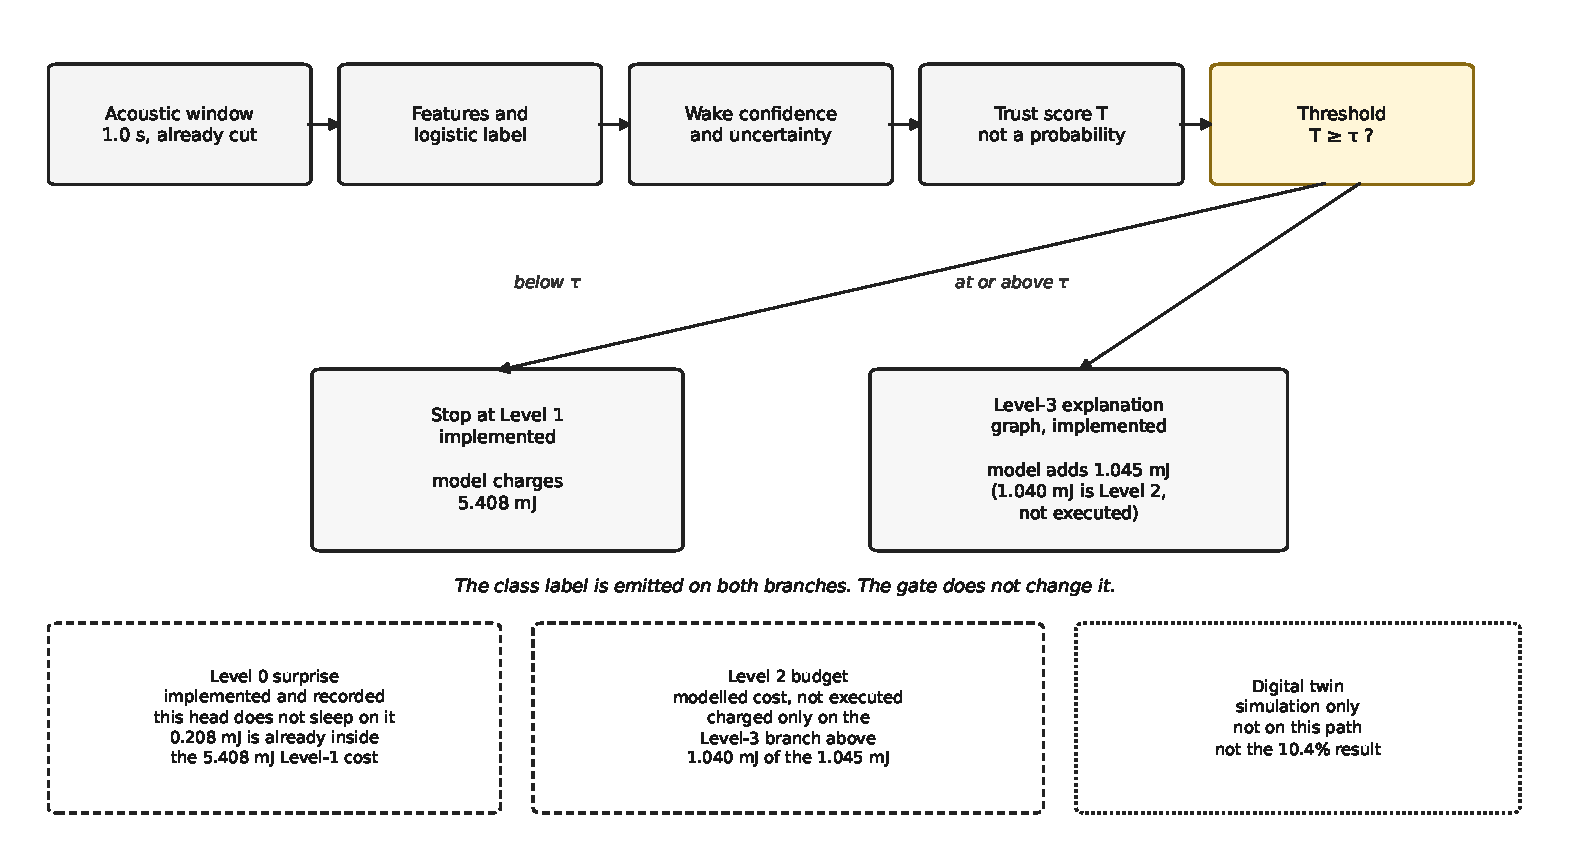
\includegraphics[width=\textwidth]{fig_architecture.pdf}
    \caption{Implemented path from a pre-segmented window to the explanation decision. Solid boxes run in the reported experiments. Joules beside the branches are the datasheet model, not a measured current. Dashed boxes are a modelled cost or a separate simulation. The logistic label is emitted on both branches.}
    \label{fig:architecture}
\end{figure}

The reported fish label is the argmax of a class-balanced logistic regression on 102 numbers: 99 log-Mel statistics (per-band mean, standard deviation, and maximum of 32 bands, plus three coarse band means) and three waveform numbers inside the band stored on the graph node \texttt{cause.taxon.opsanus\_tau}, which is 80--500\,Hz. Those three numbers are the in-band power fraction, the in-band spectral flatness, and the autocorrelation peak between lags $f_s/500$ and $f_s/80$. The bounds are read from the graph. They were not tuned on the test files. Features are standardised with the training mean and variance. The solver is lbfgs with \texttt{class\_weight="balanced"}. A small convolutional budget of 546 parameters exists in the hierarchy for a MAC count. It does not supply this label.

Validation macro-F1 on the seed-0 recording-locked split was 0.799 without the three band numbers and 0.817 with them. A multilayer perceptron on the same vector scored 0.819 and was not used. The test split did not choose the features or the estimator. The Mel-only test macro-F1 of 0.827 is a preserved comparison and is not the number in Section~\ref{sec:results}.

\begin{algorithm}[!htbp]
\caption{One-threshold explanation gate. The logistic label is emitted on both branches.}
\label{alg:gate}
\begin{algorithmic}
\Require window $i$, score $s_i$, validation-chosen threshold $\tau$
\State Fit or load the class-balanced logistic and emit $\hat{y}_i$
\If{$s_i \ge \tau$}
    \State Charge Level~3 and attach the graph explanation
\Else
    \State Stop at Level~1
\EndIf
\State \Return $\hat{y}_i$
\end{algorithmic}
\end{algorithm}

\subsection{Event-level trust estimation}\label{sec:trust}

\begin{definition}[Dirichlet lift]
Logistic probabilities $\tilde{p}$ are lifted by
\begin{equation}
\alpha_k = 1 + 20\,\tilde{p}_k, \qquad \hat{p}_k = \alpha_k \Big/ \sum_j \alpha_j.
\label{eq:lift}
\end{equation}
The concentration 20 is fixed. It is not learned.
\end{definition}

For a head with a negative class, wake confidence is $C = 1 - \hat{p}_{\mathrm{neg}}$. For the toadfish head the negative class is \texttt{other}. Aleatoric uncertainty is $u_a = 1 - \max_k \hat{p}_k$. Epistemic uncertainty is $u_e = K / \sum_k \alpha_k$. With this fixed concentration, $\sum_k \alpha_k = K + 20$, so $u_e = K/(K+20)$ on every window. For two classes, $u_e = 2/22 \approx 0.0909$.

Health consistency $\kappa$ is 1 unless the sensor report says clipping, a fault, fewer than 12 ADC bits, or a drift above 5\,ppm. Environmental consistency $\rho$ is a sigmoid of the low-band minus high-band Mel contrast, reduced by sea state and turbulence. After per-bin instance normalisation, that contrast equals the FiLM bias of the environment state. When the state is the imputed constant, $\rho$ is the same number on every window.

\begin{definition}[Event trust]
Event trust is the gate score
\begin{equation}
T = \sigma\bigl(2.2\,C + 0.8\,\kappa + 1.1\,\rho - 1.4\,(u_a + u_e) - 0.6\bigr),
\label{eq:trust}
\end{equation}
where $\sigma$ is the logistic sigmoid. The four weights and the bias do not sum to 1.
\end{definition}

$T$ is a gate score. It is not a calibrated probability that the label is correct, and it is not the convex combination $w_C C + w_E E + w_K K + w_U(1-U)$. The knowledge graph is not an input of $T$.

The coefficients are constants stored with the implementation. They were not estimated from these recordings, and no validation search selected them. The wake coefficient is the largest, so the score moves with confidence when the other inputs are fixed. Uncertainty is subtracted, so a more diffuse distribution would lower the score when that distribution varies. Health and environment have smaller positive coefficients for the case in which the sensor report or the sea state changes. The bias shifts the sigmoid. On this corpus those roles are not exercised: $\kappa = 1$, $\rho = 0.259$, and $u_e = 2/22$ on every window. Multiplying any one coefficient by $0.5$ or by $2$ left the validation percentile unchanged. The particular numbers do not create a different decision here. Any strictly increasing function of wake confidence would have selected the same windows after its own threshold was retuned.

On a two-class head, $u_a = 1 - \max(C, 1-C)$. With $\kappa$, $\rho$, and $u_e$ constant, $T$ is a strictly increasing function of $C$ at the weights above. A threshold on $T$ and a threshold on $C$ therefore rank windows in the same order. That algebraic fact is why the trust gate cannot outperform confidence on this dataset. Section~\ref{sec:ablation} is the empirical counterpart: after each score's own validation threshold is applied, the test masks match. The fixed-concentration lift does not provide a window-varying epistemic uncertainty in this two-class experiment, and it is not evidence of superior uncertainty estimation.

\subsection{Uncertainty estimation and calibration}\label{sec:calibration-method}

The concentration 20 is a constant in the code. It is not a trained parameter. Changing it re-lifts the same logistic probabilities. It does not refit the logistic. Section~\ref{sec:sensitivity} sweeps the values 5, 10, 20, and 40 on validation. The reported test rows use 20.

Two uncertainty scores are compared with the same validation rule. The Dirichlet score used as a gate is $1 - (u_a + u_e)$, so a large uncertainty is the low side of the threshold. The alternative is one minus the normalised entropy of the Dirichlet mean, $1 - H(\hat{p})/\log K$. Both are high when the mean is peaked on either class. A confident negative therefore looks like a confident positive to these two scores. Wake confidence does not make that mistake, because a confident negative has low $C$.

Calibration of $C$, of $T$, of $1-(u_a+u_e)$, and of the entropy score against the event indicator is reported with the baseline comparison in Section~\ref{sec:compare}. A lower value means the scalar is closer to a probability of the event. It does not by itself make a better gate. $T$ is not that probability.

\subsection{Cost-sensitive gating policy}\label{sec:policy}

For a score $s$, candidate thresholds are the 5th, 10th, \ldots, 95th percentiles of the validation scores. At each candidate the validation objectives, all minimised, are the mean modelled energy, the fraction of negative windows that receive Level~3, and one minus the fraction of positive windows that receive Level~3. The chosen threshold is the Chebyshev knee of that grid after min-max scaling. Ties break toward lower energy, then the earlier percentile. The frozen threshold is applied once to the test scores. Test labels do not enter the grid.

The same rule defines four scores: wake confidence, the inverted uncertainty, the confidence--uncertainty logit with the health and environment weights set to zero, and full trust. Always-Level-1 and always-Level-3 have no threshold. An optional three-threshold staircase is searched with NSGA-II \cite{deb2002} on validation only (population 12, six generations) and scored once on test. That staircase can stop at Level~0. It is not a row of the one-threshold table, and it is not the knee previously fit on the test split. That earlier knee, and the 3.82\,mJ figure attached to it, is retired.

The abstention baseline uses the same percentile grid and a different action: if the score is below its own validation threshold, the label is refused. Its objectives are the abstention rate, the error rate among accepted labels, and one minus the full-set macro-F1 when a refusal matches no gold label. It is reported separately so that a lower error on the accepted subset is not mistaken for a better classifier.

\subsection{Computational complexity and energy-cost model}\label{sec:energy}

The device row is the STM32L476 profile in the datasheet model: 80\,MHz, 8\,mW active, 2.5\,nJ per INT8 MAC. No board current was measured. MAC counts by level are $8\times 10^{4}$, $2\times 10^{6}$, $4\times 10^{5}$, $2\times 10^{3}$, and $2\times 10^{3}$ for Levels 0 through 4. Energy through a level is the cumulative MAC cost plus the active energy for the time those MACs would take. The resulting level costs are 0.208, 5.408, 6.448, and 6.453\,mJ per window for Levels 0 through 3.

For a window that runs the logistic,
\begin{equation}
E_i = E_{a,i} + E_{g,i} + E_{p,i}.
\label{eq:energy}
\end{equation}
$E_{a,i}$ is the cost through Level~1, 5.408\,mJ. $E_{g,i}$ is 0. Trust is arithmetic on quantities Level~1 already computed, and the profile has no separate trust MAC count. $E_{p,i}$ is the remainder when Level~3 is selected, 1.045\,mJ, and 0 otherwise. Of that 1.045\,mJ, 1.040\,mJ is the Level-2 budget and 0.005\,mJ is Level~3. The Level-2 share of the additional path is 0.995. The fish label does not execute that network. The cost model charges it because the energy function sums every level up to the one selected. The graph walk is the small remainder.

Average energy is the mean of $E_i$ over the $N$ test windows. The saving against always-Level-3 is
\begin{equation}
100 \times \bigl(\bar{E}_{\mathrm{L3}} - \bar{E}\bigr) / \bar{E}_{\mathrm{L3}}.
\label{eq:saving}
\end{equation}
An arrival rate is not in the model. The same rate would multiply every policy and cancel in the percentage. No arrival process was fitted.

The cumulative charge is appropriate only for a stack that actually executes every level up to the one selected. The reported logistic does not execute Level~2. The energy function still sums that level because it is present in the stack. An alternative account uses the same windows and drops the Level-2 budget, so an explanation adds only the graph walk, $0.005$\,mJ. Always attaching the graph then costs $5.413$\,mJ per window. The gated windows cost $5.410$\,mJ. The saving is $0.062\% \pm 0.004\%$ over the three seeds. Almost all of the $10.4\%$ figure is the decision to charge an unused network. This alternative is a restatement of the published energy identity. It is not a second experiment and not a measured current. The twin saving in Appendix~\ref{app:twin} is a different generator and is not this number.

\section{Experimental setup}\label{sec:setup}

\subsection{Datasets and preprocessing}\label{sec:data}

\paragraph{Toadfish.}
Clips are ToadFishFinder v4 \cite{bohnenstiehl2023data}, folders of boatwhistles and other sounds, 1.35\,s, 24\,kHz, 32-bit integer PCM. The loader takes the centre 1.0\,s and resamples to 16\,kHz. At most 3{,}000 files per class are drawn, and a deployment parsed from the file name is kept whole. Both classes of one deployment stay on one side. The split is 60/20/20 by file mass. It blocks same-recording leakage. It does not hold out a second estuary. Every station in the release is Pamlico Sound. Seed 0 uses 1{,}803/1{,}797, 615/585, and 582/618 files for other and boatwhistle, in 734, 257, and 309 groups. Seeds 1 and 2 redraw the groups. Group overlap across train, validation, and test was 0 on every seed. The events are pre-segmented. This is not end-to-end discovery in a continuous recording.

\paragraph{Noise.}
For seed 0 only, white noise is added to the test waveform before feature extraction, at 20, 10, 5, and 0\,dB, with a fixed random stream per level. The logistic and the threshold stay frozen. The bounds 80 and 500\,Hz are not retuned. This is a controlled perturbation of stored waveforms. It is not a field recording and it is not a validation of robustness at sea.

\paragraph{Watkins.}
The full-cuts archive of the Woods Hole Oceanographic Institution \cite{sayigh2016} is used under its academic terms and is not redistributed. A species enters only if it has at least 40 cuts and 8 tapes and if a 16\,kHz front end keeps the call. Sixteen species remained. At most 500 files per species were kept, whole tapes, seed 0. The tape id is the leading five digits of the trailing token. This is a call-library task on isolated cuts. It is not the toadfish task, and the macro-F1 values are not compared.

\paragraph{Twin.}
The appendix uses the seed-0 busy-strait draw, 138/32/43 windows. It is a simulation.

\subsection{Experimental protocol and parameter settings}\label{sec:protocol}

Each fish seed fits the logistic on its own training windows (\texttt{max\_iter} 2000; the fits stopped at iterations 64, 67, and 63). Every threshold in Section~\ref{sec:policy} is chosen on that seed's validation windows and applied once to its test windows. The concentration used for the test rows is 20. The weight vector is the hand-set vector in Equation~\eqref{eq:trust}. Seeds are 0, 1, and 2.

The unit of every mean, sample standard deviation, and 95\% Student interval in the fish tables is the seed-level number. The sample standard deviation uses $R-1$ in the denominator, so $R = 3$. The interval is across three redraws of the recording-locked split inside one estuary. It is not an interval over windows, over recording groups, or over a second site. Paired $t$ statistics are two-sided contrasts of those three pairs. They are descriptive. They are not evidence that a ranking will hold under new recording conditions. The trust-minus-confidence difference is zero on every test window, and therefore inside every recording group. A group-level interval on that contrast would be degenerate. Per-window scores were not archived, and no further fit was run.

The threshold is not chosen on the test set. Bands are not retuned after the test score. Species are not dropped. Temperature scaling and Cohen's kappa were not run.

\subsection{Baseline methods}\label{sec:baselines}

The one-threshold table contains always-Level-1, always-Level-3, a confidence threshold, an uncertainty threshold, a confidence--uncertainty threshold, and the trust threshold. Ablations set the environment weight or the uncertainty weight to zero and retune the threshold, or compute trust and then never run Level~3. The uncertainty comparison adds the entropy score. The abstention baseline is separate. The NSGA-II staircase is separate. The seed-0 energy-threshold ROC in Section~\ref{sec:compare} is the preserved detector from the earlier single-seed suite on the same split. This comparison did not refit it, and seeds 1 and 2 do not have that AUC.

\subsection{Evaluation metrics}\label{sec:metrics}

Classification uses macro-F1, per-class recall, and, for each seed, the confusion matrix. The error rate among accepted predictions equals the logistic error rate on every explanation-gate row, because those rows accept every label. Abstention reports both the error on the accepted subset and the macro-F1 on all windows with refusals counted as errors. Energy uses joules per window, the saving against always-Level-3, and the fraction of windows that select Level~3. Explanation recall is the fraction of true boatwhistles that receive Level~3. Explanation false alarm is the fraction of \texttt{other} windows that receive Level~3. Calibration uses expected calibration error of a score against the event indicator.

\section{Results and discussion}\label{sec:results}

\subsection{Comparative performance evaluation}\label{sec:compare}

The central comparison is in Table~\ref{tab:gates}. Trust-based gating does not outperform confidence-based gating. The two rows are identical. Macro-F1 is the logistic's and is the same on every explanation-gate row, because the gate does not change the label. Gating does not improve classification accuracy. The mean over three seeds is $0.844 \pm 0.004$ (seeds 0.839, 0.848, and 0.844). The 95\% interval is $[0.833, 0.854]$. Mean per-class recall is $0.816 \pm 0.039$ for the boatwhistle and $0.872 \pm 0.041$ for \texttt{other}. The mean error rate on all predictions is 0.156. Wake ROC-AUC is $0.908 \pm 0.009$. Wake ECE is $0.043 \pm 0.017$, with a 95\% interval $[0.000, 0.085]$ that is too wide to support a tight calibration claim.

\begin{table}[!htbp]
\centering
\caption{One-threshold gates on the toadfish test windows. Entries are mean $\pm$ sample standard deviation over seeds 0, 1, and 2. Energy is the datasheet model. A standard deviation is omitted when it is below the reported rounding, except where the text gives the seed-wise spread.}
\label{tab:gates}
\footnotesize
\setlength{\tabcolsep}{3pt}
\begin{tabular}{|l|c|c|c|c|c|c|c|}
\hline
\textbf{Method} & \textbf{Macro-F1} & \makecell{\textbf{Energy}\\\textbf{(mJ)}} & \makecell{\textbf{Saving}\\\textbf{(\%)}} & \makecell{\textbf{Level-3}\\\textbf{rate}} & \makecell{\textbf{Explain}\\\textbf{recall}} & \makecell{\textbf{Explain}\\\textbf{FA}} & \makecell{\textbf{Error on}\\\textbf{accepted}} \\
\hline
Always Level 1 & $0.844 \pm 0.004$ & 5.408 & 16.2 & 0 & 0 & 0 & 0.156 \\
\hline
Always Level 3 & $0.844 \pm 0.004$ & 6.453 & 0 & 1 & 1 & 1 & 0.156 \\
\hline
Confidence & $0.844 \pm 0.004$ & 5.779 & $10.4 \pm 0.7$ & $0.355 \pm 0.041$ & 0.662 & 0.039 & 0.156 \\
\hline
Uncertainty & $0.844 \pm 0.004$ & 5.904 & $8.5 \pm 0.7$ & 0.474 & 0.501 & 0.446 & 0.156 \\
\hline
Conf.--uncertainty & $0.844 \pm 0.004$ & 5.779 & $10.4 \pm 0.7$ & $0.355 \pm 0.041$ & 0.662 & 0.039 & 0.156 \\
\hline
Trust & $0.844 \pm 0.004$ & 5.779 & $10.4 \pm 0.7$ & $0.355 \pm 0.041$ & 0.662 & 0.039 & 0.156 \\
\hline
\end{tabular}
\end{table}

The paired difference between trust and the confidence threshold is 0 on energy, on the Level-3 rate, on explanation recall, and on explanation false alarm. A paired $t$ test is undefined for a zero difference. The uncertainty threshold spends more energy, explains fewer true boatwhistles, and explains far more negatives (observed paired contrasts $p = 0.026$, $0.032$, and $0.0009$). Those three numbers are descriptive contrasts of three seeds, not evidence of superiority on a new deployment. The entropy of the Dirichlet mean matched the uncertainty gate on every seed. Both scores are high when the distribution is peaked, including when it is peaked on \texttt{other}.

On seed 0, expected calibration error of wake confidence against the event indicator is 0.059. The same indicator gives 0.250 for inverted uncertainty, 0.160 for the entropy score, and 0.260 for trust. Trust is a worse probability of the event than wake confidence, which is expected if $T$ was not trained as a probability. Emitting an uncertainty value does not make a better explanation gate. Across seeds, wake ECE is 0.059, 0.044, and 0.025. Epistemic uncertainty was $2/22$ on every window.

Seed 0 reproduces the earlier single-seed fit. Macro-F1 is 0.839, wake ROC-AUC is 0.898, ECE is 0.059, and the Brier score is 0.120. Precision, recall, F1, and support are 0.880, 0.796, 0.836, and 618 for the boatwhistle, and 0.803, 0.885, 0.842, and 582 for \texttt{other}. The confusion matrix, rows true and columns predicted, in the order (boatwhistle, other), is $[[492, 126], [67, 515]]$. Seed 1 is $[[472, 125], [57, 546]]$. Seed 2 is $[[522, 84], [103, 491]]$.

The validation rule chose the 65th percentile of each monotone score. On seed 0 the numeric thresholds differ (trust 0.848, confidence 0.767, confidence--uncertainty 0.653, environment weight removed 0.808, uncertainty weight removed 0.898). The selected windows do not differ.

The seed-0 energy-threshold detector, preserved from the earlier suite on this same split, has ROC-AUC 0.656 against 0.898 for wake confidence. That comparison is a ranking of the event, not a row of Table~\ref{tab:gates}. Seeds 1 and 2 do not have that AUC.

\paragraph{Abstention, reported separately.}
Refusing the label when trust is below a validation threshold does not reproduce Table~\ref{tab:gates}. On seeds 0, 1, and 2 the abstention rates are 0.591, 0.627, and 0.488. The error rates among accepted labels are 0.075, 0.060, and 0.160, which are lower than the full-set error on seeds 0 and 1. Macro-F1 on the accepted subset is 0.480, 0.484, and 0.457. Macro-F1 on all windows, with refusals counted as errors, is 0.409, 0.403, and 0.423. On seed 0 the full-set recall of \texttt{other} under that scoring is 0. The rule keeps confident boatwhistle predictions and drops the negative class. The reduction in accepted error is the refusal, not a better classifier. The logistic macro-F1 on the same windows remains 0.839, 0.848, and 0.844.

\subsection{Component-wise ablation study}\label{sec:ablation}

Table~\ref{tab:ablation} is the same test protocol with one component removed at a time. ``Level 3 never'' still computes trust and then withholds the graph.

\begin{table}[!htbp]
\centering
\caption{Ablations on the toadfish test windows. Means over three seeds. A matching energy and Level-3 rate means the test mask matched the trust row after the threshold was retuned on validation.}
\label{tab:ablation}
\footnotesize
\setlength{\tabcolsep}{3pt}
\begin{tabular}{|p{3.6cm}|c|c|c|c|c|c|}
\hline
\textbf{Configuration} & \textbf{Trust} & \textbf{Unc.} & \textbf{Env.} & \textbf{Level 3} & \textbf{Macro-F1} & \makecell{\textbf{Energy}\\\textbf{(mJ)}} \\
\hline
No gate & unused & no & no & never & 0.844 & 5.408 \\
\hline
Wake only & $C$ & no & no & if $C \ge \tau$ & 0.844 & 5.779 \\
\hline
Wake and uncertainty & logit & yes & no & if score $\ge \tau$ & 0.844 & 5.779 \\
\hline
Trust, environment weight 0 & yes & yes & 0 & if $T \ge \tau$ & 0.844 & 5.779 \\
\hline
Trust, uncertainty weight 0 & yes & no & yes & if $T \ge \tau$ & 0.844 & 5.779 \\
\hline
Full trust & yes & yes & yes & if $T \ge \tau$ & 0.844 & 5.779 \\
\hline
Full trust, Level 3 never & computed & yes & yes & never & 0.844 & 5.408 \\
\hline
\end{tabular}
\end{table}

The Level-3 rate is 0 for the two rows that never explain and $0.355$ for every row that explains under a retuned threshold. The graph is not an input to $T$. When the logistic says toadfish, the attached text names \texttt{cause.taxon.opsanus\_tau} because that event has one \texttt{caused\_by} edge. The match is the wiring, not a validation of the class. A label-free band comparison has ROC-AUC $0.630 \pm 0.053$ and is not used as a check that the predicted class is correct. The graph does not change the label.

Health consistency was 1 on every window. Environmental consistency was 0.259 on every window, to numerical noise, for the reason in Section~\ref{sec:trust}. Zeroing either weight shifts the logit by a constant. The retuned percentile absorbs the shift. This ablation cannot show a field effect of sea state, because the sea state never changes, and it cannot show a spectral effect of $\rho$, because instance normalisation has already removed the clip's band means from that scalar.

\subsection{Robustness and generalisation analysis}\label{sec:robust}

\paragraph{Noise.}
Table~\ref{tab:snr} is the frozen seed-0 head and the frozen clean-validation threshold, with white noise added before the features.

\begin{table}[!htbp]
\centering
\caption{Controlled white-noise perturbation of the seed-0 test waveforms. The head and the clean-validation threshold stay frozen. These rows are not a field recording and not a sea trial.}
\label{tab:snr}
\begin{tabular}{|c|c|c|c|c|c|}
\hline
\textbf{SNR (dB)} & \textbf{Macro-F1} & \textbf{Wake ROC-AUC} & \textbf{Wake ECE} & \textbf{Boatwhistle recall} & \textbf{Level-3 rate} \\
\hline
clean & 0.839 & 0.898 & 0.059 & 0.796 & 0.362 \\
\hline
20 & 0.820 & 0.878 & 0.081 & 0.735 & 0.309 \\
\hline
10 & 0.758 & 0.831 & 0.147 & 0.595 & 0.223 \\
\hline
5 & 0.711 & 0.810 & 0.208 & 0.487 & 0.166 \\
\hline
0 & 0.608 & 0.787 & 0.280 & 0.327 & 0.077 \\
\hline
\end{tabular}
\end{table}

Boatwhistle recall falls as the noise rises. Recall of \texttt{other} rises, because the head says \texttt{other} more often. The Level-3 rate falls because the scores fall under a threshold that was chosen on clean validation.

\paragraph{Second dataset.}
The Watkins tape hold-out is seed 0 only and is a negative result, not a successful generalisation. Test macro-F1 is 0.281 against a pre-registered bar of 0.70. Accuracy is 0.285. The majority class, humpback whale, has accuracy 0.062. Seeds 1 and 2 were not run. Fin whale F1 is 0.767 and killer whale F1 is 0.692. Striped dolphin and walrus are 0.000, each one test tape, and they stay in the average. The archive mixes equipment, decades, and sites inside a species folder \cite{sayigh2016}, and the split holds the tape out \cite{aguiar2021}. It is not the BEANS random split \cite{hagiwara2022}, and 0.281 is not comparable to the toadfish macro-F1.

\paragraph{Pre-segmentation.}
Both acoustic evaluations score events that were already cut. Neither demonstrates detection in a continuous recording.

\paragraph{Level 0 on the seed-0 fish split.}
Test boatwhistles have median surprise 3.599, and all 618 sit below the twin admit point at 5.398. A pipeline that slept on that cutoff would reject every boatwhistle. The fish head records surprise and does not use it as the label.

The digital twin is a different generator. Its large simulated saving is not a result of this section. The assumptions and the secondary numbers are in Appendix~\ref{app:twin}.

\subsection{Estimated energy-cost and sensitivity analysis}\label{sec:sensitivity}

The trust gate's $10.4\% \pm 0.7\%$ is the saving of explaining about 35\% of windows instead of all of them, under the cumulative datasheet model. Always stopping at Level~1 saves 16.2\% and explains nothing. The knee trades those two objectives against explanation false alarms. On the seed-0 validation curve the 65th percentile, which is the chosen point, explains 35\% of windows, recalls 0.646 of validation boatwhistles, and false-alarms on 0.068 of validation negatives, for a validation saving of 10.5\%. The 5th percentile explains 95\% of windows and saves 0.8\%. The 95th percentile explains 5\% and saves 15.4\%. The test operating point was the validation knee, not a point read off the test curve.

Scaling the additional-path cost by 0.5, 1, 2, and 5, and retuning the threshold on validation, left the chosen percentile at 65. The validation saving moved from 5.7\% to 10.5\%, 18.1\%, and 31.9\%, because the same decisions were priced differently. Scaling only the Level-3 joules by the same factors moved the validation saving from 10.51\% to 10.70\%. The result tracks the Level-2 budget inside the cost model. It does not track the graph walk.

Scaling each hand-set weight by 0.5, 1, and 2, one at a time, left the validation percentile at 65 and left the validation explanation rates unchanged. The same was true of concentrations 5, 10, 20, and 40: epistemic uncertainty moved from 0.286 to 0.048, the numeric threshold moved, and the validation mask did not. These sweeps are validation surfaces. They were not used to pick a test-set champion. The reported test configuration remains concentration 20 and the hand-set weights.

The validation-chosen NSGA-II staircase is a different policy. On the three test sets its modelled energy is 6.07, 5.85, and 3.70\,mJ per window, with detection misses 0.105, 0.104, and 0.070. Seed 2's 3.70\,mJ sits below the Level-1 cost of 5.41\,mJ, so that policy is charging some windows as Level~0. Its energy is not comparable to Table~\ref{tab:gates}. The retired test-tuned knee at 3.82\,mJ is not this row and is not quoted as a result.

\subsection{Discussion of key findings}\label{sec:discussion}

This study examines whether uncertainty and contextual terms improve event-level explanation gating over a confidence threshold under an explicit energy-cost model. On the evaluated two-class toadfish corpus, the trust score ranks windows the same way as wake confidence, while the uncertainty-only gate is less selective. The estimated energy benefit depends on charging a Level-2 budget that does not produce the label.

The classifier that should be believed is the three-seed macro-F1 of $0.844 \pm 0.004$ on pre-segmented Pamlico candidates, with the recording held out. The gate does not change that number. Wake confidence ranks boatwhistles above the negative class better than the seed-0 energy threshold (ROC-AUC 0.898 against 0.656). The three band numbers, on an earlier comparison, removed fifteen false boatwhistles at the same true-positive count of 492. That is a small change beside a ResNet-50 on the 24\,kHz spectrogram of the same call \cite{bohnenstiehl2023}, and the splits differ.

The gate that should be believed is the confidence threshold. Trust matches it because health, environment, and epistemic uncertainty are constant and aleatoric uncertainty is a function of wake confidence. The same modelled saving, $10.4\% \pm 0.7\%$ against always-Level-3, is therefore available without the extra terms, and only under the cumulative cost model. If Level~2 is not charged, that saving falls to about $0.06\%$. An uncertainty threshold is a worse explanation policy on these files. The intervals use three seeds inside one estuary. They do not estimate a new deployment. Watkins macro-F1 of 0.281 missed 0.70 and is not generalisation. A controlled noise perturbation lowers seed-0 macro-F1 from 0.839 to 0.608 at 0\,dB. It is not a sea trial.

\section{Limitations and threats to validity}\label{sec:limits}

This study evaluates event-level trust gating using available underwater acoustic recordings and a model-based energy-cost framework. The reported energy savings are estimates derived from the specified computational assumptions and are not measurements from a physical underwater deployment. The evaluation therefore establishes the potential of the proposed decision mechanism under the tested conditions rather than demonstrating its operational performance in an underwater environment. Future work should examine the framework using embedded hardware and field measurements when suitable facilities become available.

The same limits are stated in the abstract and in Section~\ref{sec:discussion}, because they change what the main result means. The fish files are pre-segmented candidates from one estuary, so the study does not show event discovery and does not show a second site. The trust score is equivalent to confidence gating on this dataset. The $10.4\%$ figure charges a Level-2 network the label does not run. Three seed-level observations do not support a claim of superiority on new recordings. Watkins is one seed and missed its bar. The twin is a simulation. Level~4 neighbour confirmation is not reached and is not an acoustic modem. Temperature scaling was not fit.

\section{Conclusion and future work}\label{sec:conclusion}

Uncertainty and contextual terms do not improve event-level explanation gating over a confidence threshold on the two-class toadfish corpus studied here. The logistic macro-F1 is $0.844 \pm 0.004$ and is unchanged by the explanation decision. The trust score ranks windows as wake confidence does, because several of its components are constant. The uncertainty-only gate is less selective. A datasheet model estimates a $10.4\% \pm 0.7\%$ saving against always running Level~3 only when an unused Level-2 budget is charged. The clips are pre-segmented candidates from one estuary. A Watkins tape hold-out at macro-F1 0.281 does not meet a pre-registered bar of 0.70 and is not generalisation.

The useful next measurement is a cost that matches the code path that actually runs, on a device that can report current, and a recording in which sea state and sensor health are not constants. Until those exist, the energy numbers stay estimates, and the trust gate stays equivalent to a confidence threshold on the corpus studied here.

\appendix
\section{Digital-twin simulation}\label{app:twin}

The twin is not the toadfish experiment. It uses spherical spreading, Thorp absorption at a fixed 1\,kHz \cite{thorp1967}, one surface bounce, and a delay clipped at 0.5\,s. Its fish class is a 280\,Hz pulse train, not a Pamlico boatwhistle. The seed-0 busy-strait draw has 138, 32, and 43 windows. On the 43 test windows, wake ROC-AUC is 0.916, the energy-threshold AUC is 0.069, and wake ECE is 0.328. A gated policy in that run uses 0.208\,mJ per window against 6.66\,mJ for always-Level-3, about 32 times, because most simulated windows never reach the graph. A 10\,Wh scaling of those joules is about 2{,}003 days against 63 days. Both figures are datasheet scaling of a different generator. They are not a battery measurement and they are not the toadfish saving of $10.4\%$. The graph loaded for that run had 20 nodes and 21 edges. The live ontology has 31 nodes and 65 edges. The synthetic hit rate was not measured on the larger graph.

\section*{Declarations}

\subsection*{Ethical approval}
This article uses existing acoustic recordings. It contains no studies with human participants or animals performed by the authors. No sound was projected into the water.

\subsection*{Availability of data and materials}
The toadfish clips are the ToadFishFinder v4 release on Dryad (doi:10.5061/dryad.gtht76hr9) under CC0 \cite{bohnenstiehl2023data}. The Watkins Marine Mammal Sound Database is used under the academic terms of the Woods Hole Oceanographic Institution and is not redistributed \cite{sayigh2016}. The fish comparison uses recording-locked seeds 0, 1, and 2, at most 3{,}000 files per class, a class-balanced logistic with a maximum of 2{,}000 iterations, and one threshold per score chosen on that seed's validation split and frozen before the test score. The command is \texttt{uaere eval --suite review --root data/toadfish --out artifacts/paper/review\_upgrade --max-per-class 3000 --min-files 40 --steps 2000}. Per-seed tables are available from the corresponding author on reasonable request. The repository is not posted with this manuscript. Energy figures are datasheet estimates from the STM32L476 profile (80\,MHz, 8\,mW active, 2.5\,nJ per INT8 MAC), not measured current. The digital-twin windows are simulated.

\subsection*{Competing interests}
The authors have no competing interests to declare that are relevant to the content of this article.

\subsection*{Funding}
No funds, grants, or other support were received for the conduct of this study or the preparation of this manuscript. The Ministry of Earth Sciences project named in the acknowledgments is a separate listing of the corresponding author. It is not a source of these measurements and it did not support this manuscript.

\subsection*{Authors' contributions}
Rhutvik Hegde and Kalyani Manoj carried out the method, the experiments, and the draft. Shashank Mouli Satapathy supervised the work and is the corresponding author.

\subsection*{Acknowledgments}
The corresponding author's publicly listed ongoing project is ``Marine Dataset Generation and Design of Expert System for Multi-aspects Analysis of Underwater Species: Indian Scenario,'' Ministry of Earth Sciences, Government of India. That project is not the source of the measurements reported here. The corresponding author's ORCID is 0000-0002-1665-8101.

%\bibliographystyle{spbasic}
\bibliography{uaere}

\end{document}
